\documentclass{article}
\usepackage[a4paper, total={16cm, 24cm}]{geometry}
\usepackage[pdfusetitle]{hyperref}
\usepackage{url}
\usepackage[backend=biber, style=alphabetic, sorting=none]{biblatex}
\addbibresource{main.bib}
\nocite{*}
\usepackage[usenames, dvipsnames, svgnames, x11names]{xcolor}
\usepackage{listings}
\usepackage{lstcoq}
\usepackage{tikz}
\usetikzlibrary{matrix}
\usetikzlibrary{arrows.meta}
\tikzstyle{matrix_node} = [matrix of nodes, nodes={draw, minimum size=20, fill=blue!10, anchor=center}, nodes in empty cells]
\tikzstyle{arrow} = [[-{>[length=7, width=5]}]
\newenvironment{no_space_center}
    {\parskip=0pt\par\nopagebreak\centering}
    {\par\noindent\ignorespacesafterend}
\newenvironment{no_padding_center}
    {\parskip=0pt\par\nopagebreak\centering}
    {\par\noindent}
\title{Implementation and verification of a data structure using dependent types}
\author{Anton Danilkin}
\begin{document}

\begin{no_space_center}
    \begin{minipage}{10cm}
        \maketitle
    \end{minipage}
\end{no_space_center}

\begin{abstract}
    
\end{abstract}

\vspace{10cm}

\section{Introduction}

One of the most important data structures in functional programming are singly linked lists, which support prepending an element in the beginning, as well as destructing a non-empty list into its head (first element) and tail (the list containing the rest of elements). Conversely, arrays are frequently used in imperative programming; they support getting and setting an element by its index, as well as, in case of vectors, dynamic resizing.

The problem of lists is that the operation of retrieving or updating an element at a specific index has linear spacial complexity in term of the size. On the flip side, operations on arrays and vectors mutate the instance they work on, which not only makes reasoning about program behavior harder, but also means that older versions of the data structure become unaccessible for future use. One way to fix that would be making a copy before each operation, but the again would mean that now everything has linear complexity.

This way the following question arises: is it possible to have a data structure that combines the benefits of singly linked lists and vectors?

\section{Similarities between numbers and lists}

Here are some standard definitions of Peano natural numbers and lists, as well as operations on them in Coq:

\begin{no_padding_center}
    \begin{tabular}{c c}
        \begin{coq}
Inductive nat :=
  | O : nat
  | S : nat -> nat.




Definition pred (n : nat) : nat :=
  match n with
  | O => O
  | S n' => n'
  end.

Fixpoint plus (n1 n2 : nat) : nat :=
  match n1 with
  | O => n2
  | S n1' => S (plus n1' n2)
  end.
        \end{coq} &
        \begin{coq}
Inductive list A :=
  | nil : list A
  | cons : A -> list A -> list A.

Arguments nil {A}.
Arguments cons {A} x l.

Definition tl {A} (l : list A) : list A :=
  match l with
  | nil => nil
  | cons _ l' => l'
  end.

Fixpoint app {A} (l1 l2 : list A) : list A :=
  match l1 with
  | nil => l2
  | cons x l1' => cons x (app l1' l2)
  end.
        \end{coq}
    \end{tabular}
\end{no_padding_center}

As remarked by Chris Okasaki \cite{okasaki_1998}, there is a clear resemblance between them: the only real difference is that \coqinline{list A} holds a datum of type \coqinline{A}, where as \coqinline{nat} does not. Here is how the list \coqinline{[7; 5; 9]} and the number 3 (which is the length of the list) could be represented:

\begin{no_padding_center}
    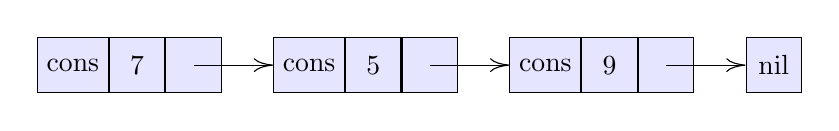
\begin{tikzpicture}
        \matrix (node1) [matrix_node, anchor=north west] at (0, 0) {
            \coqinlinelight{cons} & 7 & \\
        };
        \matrix (node2) [matrix_node, anchor=north west] at (3, 0) {
            \coqinlinelight{cons} & 5 & \\
        };
        \matrix (node3) [matrix_node, anchor=north west] at (6, 0) {
            \coqinlinelight{cons} & 9 & \\
        };
        \matrix (node4) [matrix_node, anchor=north west] at (9, 0) {
            \coqinlinelight{nil} \\
        };
        \draw [arrow] (node1-1-3.center) to (node2-1-1);
        \draw [arrow] (node2-1-3.center) to (node3-1-1);
        \draw [arrow] (node3-1-3.center) to (node4-1-1);
    \end{tikzpicture}

    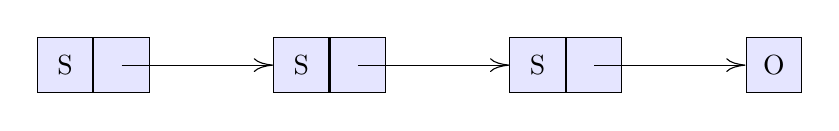
\begin{tikzpicture}
        \matrix (node1) [matrix_node, anchor=north west] at (0, 0) {
            \coqinlinelight{S} & \\
        };
        \matrix (node2) [matrix_node, anchor=north west] at (3, 0) {
            \coqinlinelight{S} & \\
        };
        \matrix (node3) [matrix_node, anchor=north west] at (6, 0) {
            \coqinlinelight{S} & \\
        };
        \matrix (node4) [matrix_node, anchor=north west] at (9, 0) {
            \coqinlinelight{O} \\
        };
        \draw [arrow] (node1-1-2.center) to (node2-1-1);
        \draw [arrow] (node2-1-2.center) to (node3-1-1);
        \draw [arrow] (node3-1-2.center) to (node4-1-1);
    \end{tikzpicture}
\end{no_padding_center}

In fact, we can go from a list to the corresponding natural number by getting its length, and back from a natural number to one of the corresponding lists by repeating an element that many times:

\begin{no_padding_center}
    \begin{tabular}{c c}
        \begin{coq}
Fixpoint length {A} (l : list A) : nat :=
  match l with
  | nil => O
  | cons _ l' => S (length l')
  end.
        \end{coq} &
        \begin{coq}
Fixpoint repeat {A} (x : A) (n : nat) : list A :=
  match n with
  | O => nil
  | S n' => cons x (repeat x n')
  end.
        \end{coq}
    \end{tabular}
\end{no_padding_center}

\printbibliography

\end{document}
